\documentclass[a4paper,11pt]{ltjsarticle}
\usepackage{luatexja}
\usepackage{luatexja-fontspec}
\usepackage{amsmath,amssymb,amsthm}
\usepackage{mathtools}
\usepackage{tikz}
\usepackage{tikz-cd}
\usepackage{geometry}
\geometry{margin=28mm}
\makeatletter
\@ifundefined{minLayer}{\DeclareMathOperator\minLayer{minLayer}}{}
\makeatother

\title{順序論における構造塔の基本例}
\author{CODEX (OpenAI)（TeX生成）\\CODEX (OpenAI)（Leanファイル生成）}
\date{\today}

\theoremstyle{definition}
\newtheorem{definition}{定義}
\newtheorem{example}{例}
\newtheorem{remark}{注意}

\begin{document}

\maketitle

\section{イントロダクション}

構造塔 (\emph{Structure Tower}) はニコラ・ブルバキ『数学原論』の精神に基づき、集合に層構造とその最小層を明示する枠組みです。本稿では Lean ファイル \texttt{OrderTheory\_Examples.lean} で構成した内容を学部生向けに解説し、主イデアルや自然数の整除順序を通して順序論的視点から構造塔を可視化します。

\section{主イデアルによる構造塔}

\begin{definition}[主イデアル]
半順序集合 $(\alpha,\leq)$ と $a\in \alpha$ に対し、
\[
  \downarrow a \coloneqq \{\,x\in \alpha \mid x \leq a\,\}
\]
を $a$ の主イデアルと呼びます。Lean 実装では
\[
  \texttt{principalIdeal}\;(\alpha)\;a = \{x \mid x \leq a\}
\]
と定義されています。
\end{definition}

主イデアルは上位元が決まると包含関係により自然な順序が得られます。Lean では
\[
  \texttt{principalIdealTower} : \alpha \mapsto \text{StructureTowerWithMin}
\]
とし、被覆性（各元がどこかの主イデアルに属する）、単調性（$i\leq j$ なら $\downarrow i \subseteq \downarrow j$）、最小層（元 $x$ に対し $\minLayer(x)=x$）を確認しています。

\section{自然数の約数による構造塔}

自然数全体 $\mathbb{N}$ を整除関係で順序づけると、$i\leq j$ は $i\mid j$ を意味します。Lean では添字集合 $\mathrm{NatDiv}$ に対し
\[
  i \leq j \iff i \mid j,\qquad i < j \iff \bigl(i \mid j\bigr)\land \neg\bigl(j \mid i\bigr)
\]
を持つ前順序を構成しました。

\begin{definition}[約数層]
自然数 $n$ に対し
\[
  L_n \coloneqq \{\,k\in \mathbb{N} \mid k\mid n\,\}
\]
とおくと、$(\mathbb{N}, (L_n)_{n\in \mathbb{N}})$ は構造塔のデータを満たします。Lean では
\[
  \texttt{StructureTowerWithMin.mk}\;\mathbb{N}\;\mathrm{NatDiv}\; (n \mapsto L_n)
\]
という形で導入されています。
\end{definition}

被覆性は任意の $x$ に対し $x\in L_x$ が成り立つことで従います。単調性 $i\mid j \Rightarrow L_i \subseteq L_j$ も整除性の推移性から明らかです。最小層は恒等写像 $\minLayer(x)=x$ としたとき $x\in L_x$ であり、$x\in L_n$ なら $x\mid n$ より $x \leq n$（整除順序）が従います。

\begin{figure}[htbp]
  \centering
  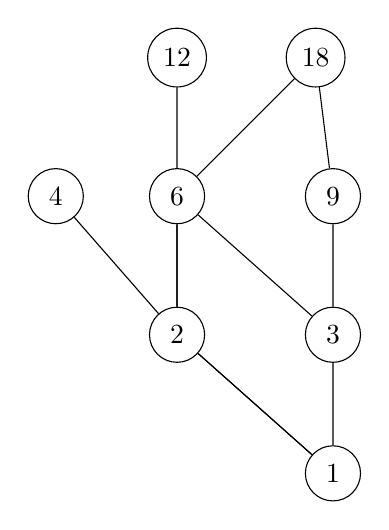
\begin{tikzpicture}[scale=1.1, every node/.style={circle, draw, minimum size=7mm}]
    \node (1) at (0,0) {1};
    \node (2) at (-1.8,1.6) {2};
    \node (3) at (0,1.6) {3};
    \node (4) at (-3.2,3.2) {4};
    \node (6) at (-1.8,3.2) {6};
    \node (9) at (0,3.2) {9};
    \node (12) at (-1.8,4.8) {12};
    \node (18) at (-0.2,4.8) {18};
    \draw (1)--(2)--(4);
    \draw (1)--(2)--(6)--(12);
    \draw (1)--(3)--(6);
    \draw (3)--(9)--(18);
    \draw (2)--(6)--(18);
  \end{tikzpicture}
  \caption{整除関係で見た自然数の層（例として $1,2,3,4,6,9,12,18$）}
  \label{fig:divisibility}
\end{figure}

図\ref{fig:divisibility} は整除関係の Hasse 図で、頂点 $n$ の上にある点は $n$ の倍数を表します。層 $L_{12}$ は路の下に現れる全ての整数を含み、最小層 $\minLayer(6)=6$ が可視化されています。

\section{フィルターと凸集合への展望}

構造塔はフィルターや凸集合とも自然に結びつきます。

\begin{itemize}
  \item \textbf{主フィルター}: 反対順序を考えると $\uparrow a = \{x \mid a \leq x\}$ は主フィルターとなり、主イデアルの双対として構造塔を構成できます。
  \item \textbf{順序凸集合}: 集合 $S$ が「$a,c\in S$ かつ $a\leq b\leq c$ なら $b\in S$」を満たすとき、$S$ は順序凸であり、凸集合の包含による塔が得られます。
\end{itemize}

これらのテーマは Lean ファイルのコメントにも「練習問題」として提示されており、主イデアル塔と同様の手法で実装を拡張できます。

\section{まとめ}

主イデアルと整除順序は、構造塔の axioms（被覆性・単調性・最小層）を具体的に満たす最初の教材になります。Lean による形式化は、証明過程を機械的に検証する良い演習であり、Lua\LaTeX{} での可視化と併せて学ぶことで順序構造の直感と厳密性を両立できます。

\end{document}
